%----------------------------------------------------------------------------------------
%	TITLE OF THE HOMEWORK	
%----------------------------------------------------------------------------------------
{\setlength{\parindent}{0pt}
\title{file title} % Article title
\fancyhead[C]{}
\begin{minipage}{0.295\textwidth} % Left side of title section
\raggedright
Math explanation\\ % Your lecture or course
\footnotesize % Authors text size
%\hfill\\ % Uncomment if right minipage has more lines
Victoria Castor-Villegas % Your name, your matriculation number
\medskip\hrule
\end{minipage}
\begin{minipage}{0.4\textwidth} % Center of title section
\centering 
\large % Title text size
Linear and Polynomial\\ % Assignment title and number
\normalsize % Subtitle text size
Regression\\ % Assignment subtitle
\end{minipage}
\begin{minipage}{0.295\textwidth} % Right side of title section
\raggedleft
\today\\ % Date
\footnotesize % Email text size
%\hfill\\ % Uncomment if left minipage has more lines
vcastorv@gmail.com % Your email
\medskip\hrule
\end{minipage}
}
%----------------------------------------------------------------------------------------
%	HOMEWORK CONTENTS
%----------------------------------------------------------------------------------------

\section{\textbf{Mathematical background}}

\subsection{Linear Regression}

Using minima squares is possible to compute a straight line that approximate in the best way all
point given, where that line is described by $y=mx+b$. That before, for at least
three pair of points.

To compute the values of $m$ and $b$ we follow the next equations (deductions left to
the reader):

\begin{align}
m = \frac{N\displaystyle\sum_{i=1}^{N}x_iy_i - \left(\sum_{i=1}^N x_i\right)\left(\sum_{i=1}^N y_i\right)}{N\displaystyle\sum_{i=1}^N x^2_i - \left(\sum_{i=1}^N x_i\right)^2}
\end{align}

\begin{align}
b = \frac{\left(\displaystyle\sum_{i=1}^N y_i\right)\left(N\displaystyle\sum_{i=1}^N x^2_i\right) -
\left(\displaystyle\sum_{i=1}^N x_i\right)\left(\displaystyle\sum_{i=1}^N x_i y_i\right)}{N\displaystyle\sum_{i=1}^N x^2_i - \left(\sum_{i=1}^N x_i\right)^2}
\end{align}

How the line approximate the numbers given is measured by the factor $r$, and when its is equal to
1 all values are described by the line. That factor can be computed by:

\begin{align}
r = \frac{\displaystyle\sum_{i=1}^N x_iy_i - N^{-1}\left(\displaystyle\sum_{i=1}^N x_i\right)\left(\displaystyle\sum_{i=1}^N y_i\right)}{\sqrt{\left[\displaystyle\sum_{i=1}^N x^2_i - N^{-1}\left(\displaystyle\sum_{i=1}^N x_i\right)^2\right]\left[\displaystyle\sum_{i=1}^N y^2_i - N^{-1}\left(\displaystyle\sum_{i=1}^N y_i\right)^2\right]}}
\end{align}

When the $r$ is not 1 (majority of cases) is useful know the uncertainties for $m$ and $b$, which can
be computed by:
\small

\begin{align}
u_m = \sqrt{\frac{N\displaystyle\sum_{i=1}^N (y_i -mx_i -b)^2}{(N-2)\left[N\displaystyle\sum_{i=1}^N x^2_i - \left(\sum_{i=1}^N x_i\right)^2\right]}}
\end{align}

\begin{align}
u_b = \sqrt{\frac{\left[\displaystyle\sum_{i=1}^N (y_i -mx_i -b)^2\right]\left[\displaystyle\sum_{i=1}^N x_i^2\right]}{(N-2)\left[N\displaystyle\sum_{i=1}^N x^2_i - \left(\displaystyle\sum_{i=1}^N x_i\right)^2\right]}}
\end{align}

\normalsize
\subsection{Polynomial Regression}

It is also know that given $n+1$ pair points is possible to compute a polynomial curve at $n^{\mathrm{tm}}$ grade that
satisfies all the pairs. Also is computable a $n-m$ polynomial regression with $m<n$, where the approach of the points
by the curve can be modified in way of the grade polynomial.

Given $n$ pairs: $\{ (x_1, y_1), (x_2, y_2), ..., (x_m, y_m)\}$ a polynomial regression can be computed as:
$y = a_nx^n + a_{n-1}x^{n-1} + ... + a_2 x^2 + a_1x + a_0$

\noindent where the coefficients are determined by the following system of linear equations.

\begin{align}
\begin{matrix}
na_0             & + & (\sum x_i)a_1       & + & (\sum x_i^2)a_2     & +...+ & (\sum x_i^n)a_n     & = & \sum y_i       \\
(\sum x_i)na_0   & + & (\sum x_i^2)a_1     & + & (\sum x_i^3)a_2     & +...+ & (\sum x_i^{n+1})a_n & = & \sum x_i y_i   \\
(\sum x_i^2)na_0 & + & (\sum x_i^3)a_1     & + & (\sum x_i^4)a_2     & +...+ & (\sum x_i^{n+2})a_n & = & \sum x_i^2 y_i \\
                 &   &                     &   &                     &       &                     & \vdots &           \\
(\sum x_i^n)na_0 & + & (\sum x_i^{n+1})a_1 & + & (\sum x_i^{n+2})a_2 & +...+ & (\sum x_i^{2n})a_n  & = & \sum x_i^n y_i
\end{matrix}
\end{align}

Therefore, is possible to solve polynomial regression by solving the linear system.

\section{\textbf{Code}}

The two cases described above are in two different files (\texttt{linear.f90}
and \texttt{polynomial.f90}). The first one about a linear regression was easy
to code since all expression are fixed. Doing the additions by \texttt{DO}
loops and the square root is a native function in \texttt{fortran} was not
necessary import any library.

For the second case, about the polynomial regression the code is little bit
more complicated, since is necessary not only a solver for the linear equation,
is also necessary compute the values for the linear system. Then, was written
two \texttt{SUBROUTINES}, one for compute the values and another one to solve
the system.

Before compute, there are a conditional to know if the system can be solved or not,
if not the program stops and gives a suggestion for a better try.

\section{\textbf{Examples}}

We can do a polynomial regression with the next pairs:
$i$) (1,1), (2,4), (3,4), (5,1), (6,2), and
$ii$) (-3,4), (-1,1), (0,0), (1,2), (2,5). At 3th grade we have:

\begin{figure}[h]
    \begin{minipage}[t]{0.5\textwidth}
      \centering
      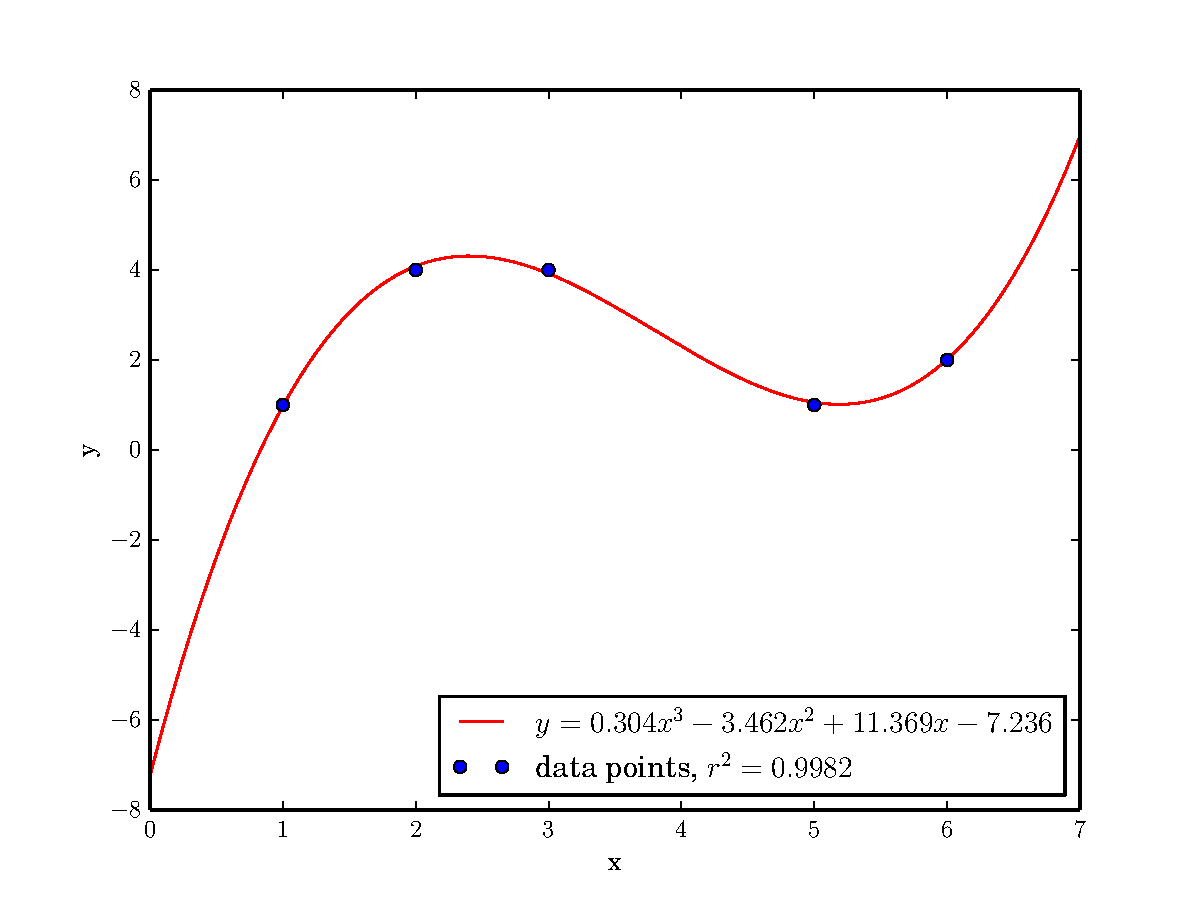
\includegraphics[width=\textwidth]{./img/6}
      \caption{Example $i$.}
    \end{minipage}%
    \hfill
    \begin{minipage}[t]{0.5\textwidth}
      \centering
      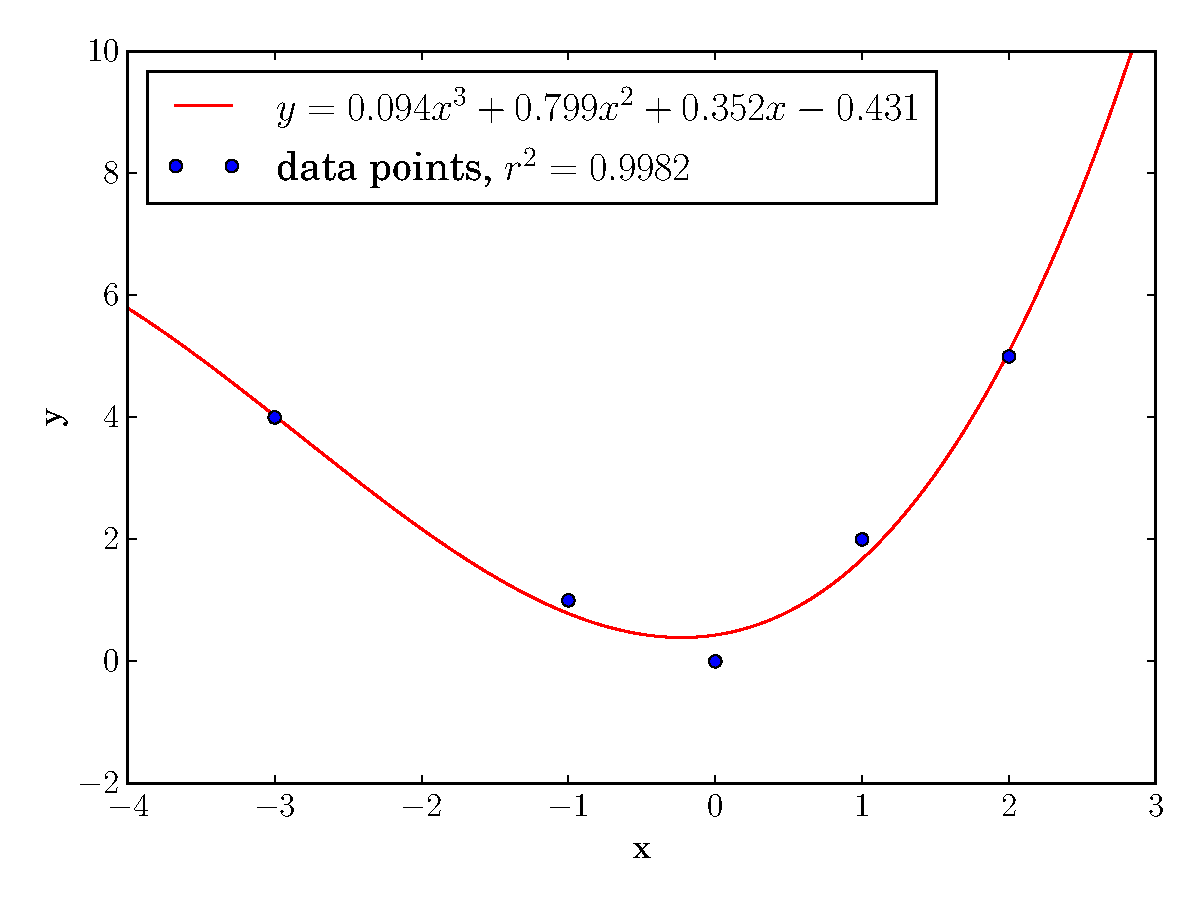
\includegraphics[width=\textwidth]{./img/7}
      \caption{Example $ii$.}
    \end{minipage}%
\end{figure}

Also we can compute for: ($-\pi/2$, 0), ($-\pi/3$, 1/2), (0, 1), ($\pi/3$, 1/2), ($\pi/2$, 0). And
compare with the function $cos(\pi/4)$. Getting a approximation of the Taylor
expansion for $cos(x)$.

$$
\cos(x) = \sum_{n=0}^{\infty}(-1)^{n}\frac{x^{2n}}{(2n)!} =
1 - \frac{x^2}{2!} + \frac{x^4}{4!} - \cdots \approx
0.966 - 0.397x^2
$$

\begin{figure}[h]
    \centering
    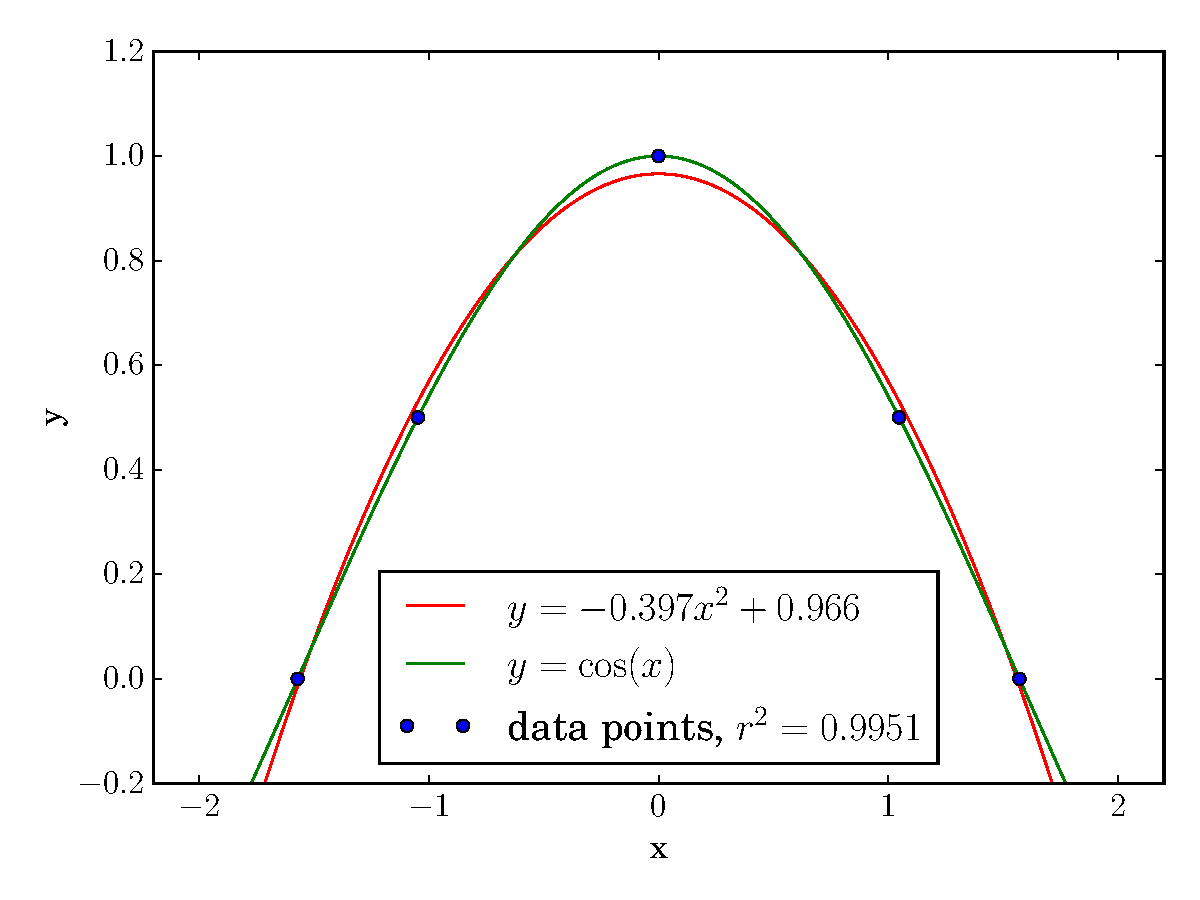
\includegraphics[width=0.70\textwidth]{./img/pi}
    \caption{Example $iii$.}
\end{figure}

